\subsection{Research Objectives and Anticipated Results}

\begin{figure}[t]
    \centering
    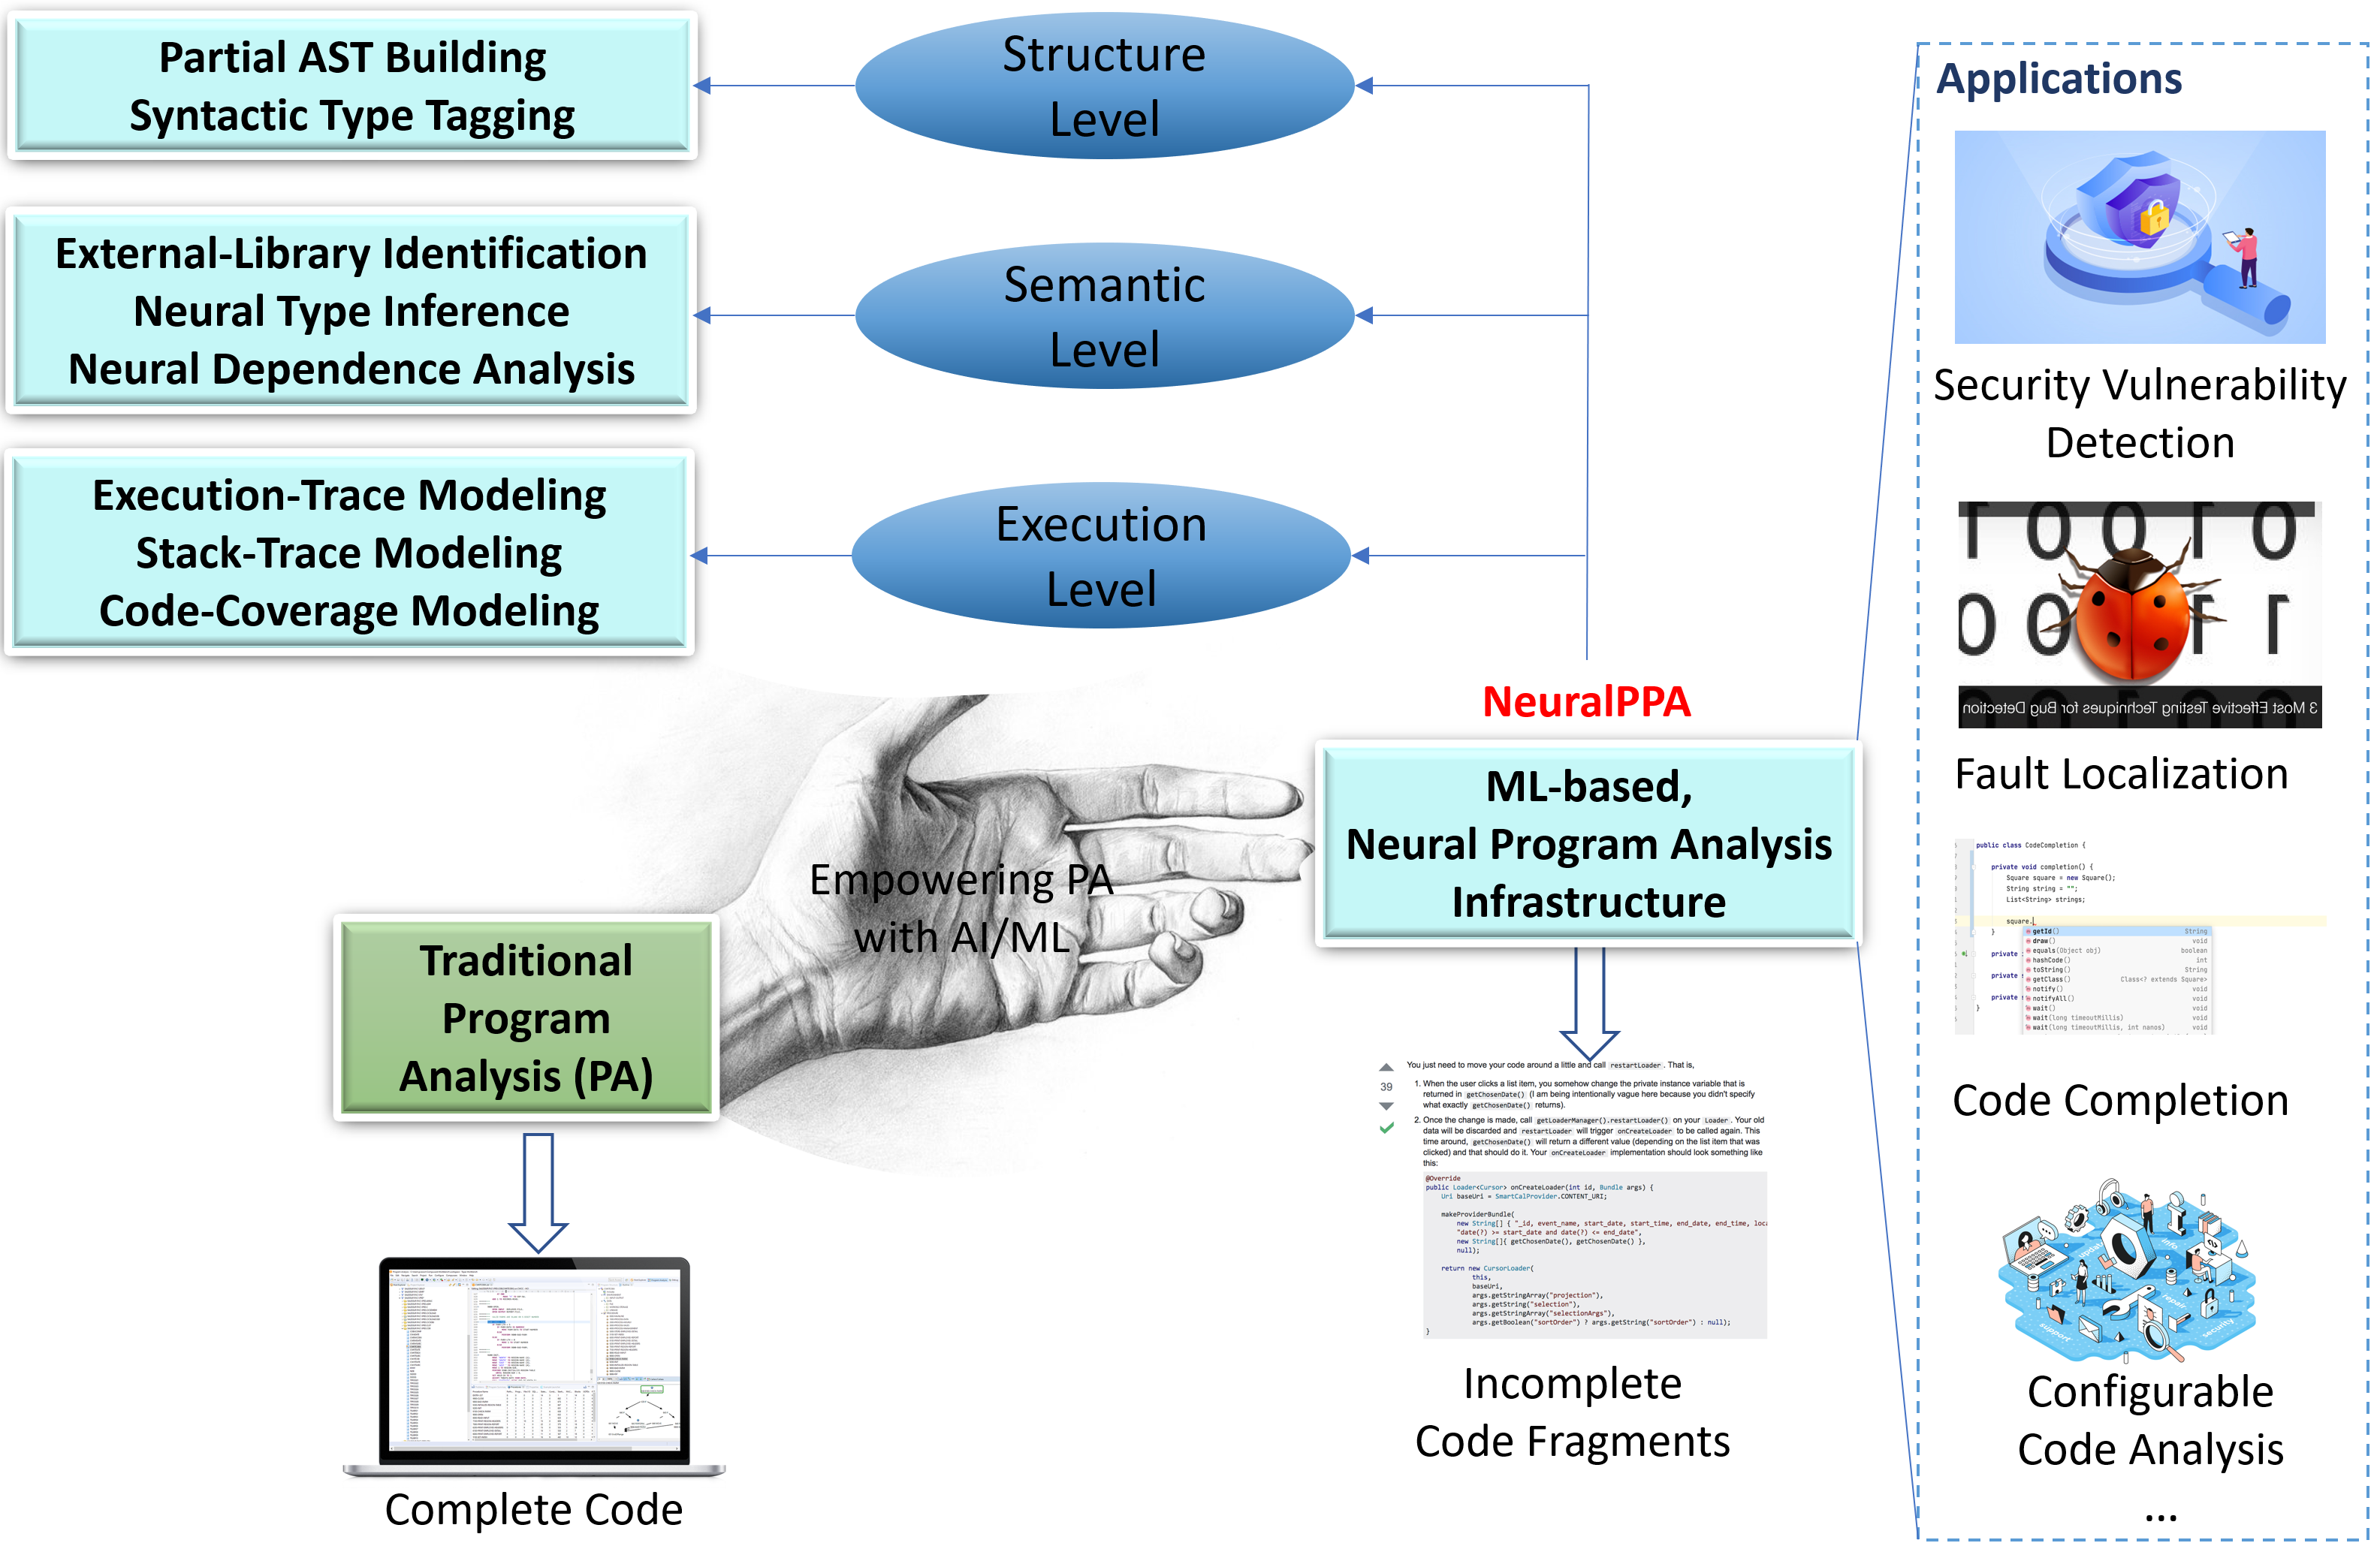
\includegraphics[width=0.9\textwidth]{graphs/neuralppa}
    \vspace{-12pt}
    \caption{{\tool}: Machine Learning-based Program Analysis Infrastructure}
    \label{fig:arch}
\end{figure}


While the state-of-the-art research and practice has been
well-established for the analysis of the entire programs, very little
research and knowledge has been achieved for partial program
analysis.
%
In this proposal, we set out to investigate and develop {\tool}, a
{\em \underline{Neural}-network-based \underline{P}artial
  \underline{P}rogram \underline{A}nalysis infrastructure}. We aim to
develop {\bf a scientific foundation, novel methodologies, frameworks,
  models, and algorithmic solutions for neural partial program
  analysis}. {\tool} {\bf enpowers program analysis (PA) with advanced
machine learning (ML) and artificial intelligence (AI) to enable the
program analysis on incomplete code fragments} (Figure~\ref{fig:arch}).
{\tool} will allow the constructions of the program analysis
techniques for partial code on which downstream software
engineering applications can be built.


Our key philosophy is that {\em the analysis of partial code can be
  learned from the analysis of entire programs in the wealth of
  information from ultra-large-scale, open-source software
  repositories}.



Specifically, we draw our motivation for such a data-driven,
learning-based approach from the following. First, ultra-large-scale
software repositories, e.g. GitHub (7M+ projects) and SourceForge
(700k+ projects) contain an enormous collection of programs. These
repositories amount to 1,000,000,000+ lines of code, 10,000,000+
revision logs, and 3,000,000+ issue reports. This wealth of knowledge
is an excellent source for {\tool}. Hindle {\em et
  al.}~\cite{naturalness-icse12} have shown that code has high
repetitiveness and predictability, and can be captured well by
statistical models. Thus, we expect to build ML models to learn from
those repositories. Second, in an empirical study on the
repetitiveness, containment, and composability of PDGs in open-source
projects, the PI group~\cite{msr16} reported that among 17.5M PDGs
with 1.6B PDG subgraphs, 14.3\% of the PDGs have all of their
subgraphs repeated across different projects. Furthermore, in 15.6\%
of the PDGs, at least 90\% of their subgraphs are likely to have
appeared before in other projects. Thus, {\tool} could learn from PDGs
with complete program dependencies retrieved from existing code
repositories and derive the dependencies for the (partial) code
fragment under study. The PI group also reported a high
repetitiveness level for AST code structure in open-source
projects~\cite{icse15}. Finally, such a program analysis
infrastructure like {\tool} can be drawn from the spirit and successes
of the approaches in natural language processing (NLP). For example,
at the lexical level, the task of deriving the token types for source
code tokens could be analogous to the part-of-speech (PoS) tagging in
NLP. At the syntax level, the task of learning the syntactic structure
in AST of the partial code can be inspired by the approaches to build
parse trees for natural-language texts. At the semantic level, the
partial program dependence analysis infrastructure is similar in
spirit to the the neural network-based dependency parsing in NLP,
which learns the dependencies signifying the semantic relationships
between words in a sentence from text corpora.

Toward this theme, in our preliminary work, we developed DeepPDA, a neural
network-based partial program dependence analysis approach that learns
to derive the program dependencies for any code fragments (i.e., both
complete and incomplete). In our preliminary empirical evaluation, we
intrinsically evaluated it on Java and C/C++ programs. First, we
trained {\tool} on complete code. For testing, we treated each method
individually and chose a consecutive portion within the method to
predict the program dependencies, and compared them against the actual
dependencies. Overall, DeepPDA predicts CFG and PDG edges in Java
with an F-score of 94.29\%, and in C++ with an F-score of
92.46\%.
%
We also developed as an approach to derive the data
types of the variables in the code snippets. We treat the problem as
statistical machine translation from source code with partially
qualified names to source code with FQNs of the APIs. Our empirical
evaluation on real-world code and StackOverflow posts shows that our
technique achieves high accuracy with 97.6\% precision and 96.7\%
recall in deriving data types in code snippets.







In {\tool}, we propose the following thrusts of research
(Table~\ref{tab:milestones}):

\vspace{3pt}
\noindent \textbf{Thurst 1. ...} ({\em Section~\ref{}}) ...


\begin{table*}[t]
	\vspace{-15pt}
\begin{center}
{\footnotesize{
\begin{tabular}{cc}
\begin{tabular}[t]{|p{0.2in}|p{2.95in}|} 
\hline
\multicolumn{2}{|>{\columncolor[gray]{0}}c|}{\textcolor{white}
{\bf Year 1 Project Milestones \& Deliverables}}\\
\hline 
\hline
\multicolumn{2}{|c|}{\bf T1. Neural Structure Analysis Infrastructure}\\
\hline
{\bf 1.1} & Neural Syntactic Type Tagging\\
{\bf 1.2} & Neural Partial AST Building\\
{\bf 1.3} & Evaluation of the components\\
\hline
\hline
\multicolumn{2}{|c|}{\bf T2. Neural Semantic Analysis Infrastructure}\\ 
\hline
{\bf 2.1} & External-Library Identification\\
\hline
%\hline
%\multicolumn{2}{|c|}{\bf Integrate Code Synthesis into Tools}\\
%\hline
%{\bf 1.5} & \goalOneFour.\\
%\hline
\multicolumn{2}{c}{}
\end{tabular}
&
\begin{tabular}[t]{|p{0.2in}|p{2.95in}|} \hline
\multicolumn{2}{|>{\columncolor[gray]{0}}c|}{\textcolor{white}
{\bf Year 2 Project Milestones \& Deliverables}}\\
\hline 
\hline
\multicolumn{2}{|c|}{\bf T2. Neural Semantic Analysis Infrastructure}\\
\hline
{\bf 2.2} & Neural Type Inference\\
{\bf 2.3} & Neural Dependence Analysis\\
%{\bf 2.3} & Integrate Evaluation Framework into Design Environment\\
%{\bf 2.4} & Evaluate CRL Framework with Existing Models\\
%{\bf 2.3} & \goalTwoThree.\\

\hline
\hline
\multicolumn{2}{|c|}{\bf T3. Neural Execution Analysis}\\ 
\hline
%{\bf 3.1} & Design New Code Representations and Learning Models.\\
{\bf 3.1} & Neural Execution-Trace Modeling\\
%{\bf 2.4} & Advance FL and RT-CI Approaches.\\
%{\bf 2.5} & Advance Regression Testing in CI Approaches.\\
%{\bf 2.5} & Advance APR Approaches with Framework.\\
\hline
%\hline
%\multicolumn{2}{|c|}{\bf Community Involvement: Capacity Building}\\
%\hline
%{\bf 2.4} & \goalTwoFour.\\
%{\bf 2.5} & \goalTwoFive.\\
%{\bf 2.6} & \goalTwoSix.\\
%\hline
\multicolumn{2}{c}{}
\end{tabular}
\end{tabular}\\
\vspace*{-.3cm}
\begin{tabular}{c}\hline
\multicolumn{1}{|>{\centering\columncolor[gray]{0}}p{6.44in}|}{\textcolor{white}
{\bf Year 3 Project Milestones \& Deliverables}}\\
\hline
\end{tabular}\\
\vspace*{-.2cm}
\begin{tabular}{cc}
\begin{tabular}[t]{|p{0.2in}|p{2.95in}|}
\hline
\multicolumn{2}{|c|}{\bf T3. Neural Execution Analysis}\\
\hline
{\bf 3.2} & Neural Stack Trace Modeling\\
{\bf 3.3} & Neural Code Coverage Modeling\\

%{\bf 3.3} & Testing on Models in IDE tools.\\
\hline
%\hline
%\multicolumn{2}{|c|}{\bf \goalTwo}\\ 
%\hline
%{\bf 3.3} & \goalThreeThree.\\
%\hline
\multicolumn{2}{c}{}
\end{tabular}
&
\begin{tabular}[t]{|p{0.2in}|p{2.95in}|}
\hline
\multicolumn{2}{|c|}{\bf T4. Neural Partial Program Analysis Applications}\\
\hline
%{\bf 3.1} & Design New Code Representations\\

{\bf 4.1} & Security Vulnerablity Detection with {\tool}\\
{\bf 4.2} & Fault Localization and Completion with {\tool}\\

\hline
\multicolumn{2}{c}{}
\end{tabular}
\end{tabular}
\vspace{-15pt}
}}
\end{center}
\vspace*{-.3in}
%\caption{Tasks and Milestones. (Rep. = Representation)}
\caption{The 3-year schedule of Thrusts, Tasks, and Milestones of this proposal.}
%the schedule of Thrusts, Tasks, and Milestones of this proposal.
%\vspace{-10pt}
\label{tab:milestones}
\vspace{-10pt}
\end{table*}
%



